\documentclass{beamer}

\usepackage{style/ufsc}
\usepackage{tikz}
\usepackage{quantikz}
\usepackage{amsmath}
\usepackage{graphicx}

\graphicspath{{./figuras/}}
\definecolor{darkgreen}{RGB}{6,128,40}

\titulo{Simulação Quântica Via QMDD}
\autores{Gabriel Sartori Rangel}
\universidade{Universidade Federal de Santa Catarina}

\begin{document}

\capa

\begin{frame}{Motivação}
  \begin{block}{Desempenho Quântico}
    \centering
    \begin{tabular}{lc}
      \textbf{Busca em lista desordenada} & \textbf{Complexidade} \\
      Clássica & $O(n)$ \\
      Quântica (Grover) & $O(\sqrt{n})$
    \end{tabular}
  \end{block}

  \begin{block}{Hardware Quântico}
    \begin{itemize}
      \item Inacessível e de baixa capacidade
      \item Equivalente à computação clássica
    \end{itemize}
  \end{block}

  Logo, algoritmos quânticos devem ser simulados em computadores clássicos.
\end{frame}

\begin{frame}{Computação quântica circuital}
  Um qubit é representado por um vetor em $\mathbb{C}^{2}$:

  \[
    \ket{\psi}
    =
    \begin{bmatrix}
      \alpha \\
      \beta
    \end{bmatrix},
    \qquad
    |\alpha|^{2}+|\beta|^{2}=1.
  \]

  Operações sobre qubits são descritas por matrizes unitárias:
  \[
    X=
    \begin{bmatrix}
      0&1\\
      1&0
    \end{bmatrix},
    \qquad
    H=\frac{1}{\sqrt{2}}
    \begin{bmatrix}
      1&1\\
      1&-1
    \end{bmatrix}.
  \]
\end{frame}

\begin{frame}{O problema do crescimento exponencial}
  \begin{columns}[c]
    \begin{column}{.48\textwidth}
      Uma operação sobre dois qubits combina matrizes pelo produto tensorial:
      \[
        X\otimes H
        =\frac{1}{\sqrt{2}}
        \begin{bmatrix}
          0&0&1&1\\
          0&0&1&-1\\
          1&1&0&0\\
          1&-1&0&0
        \end{bmatrix}.
      \]

      Duas matrizes $2\times2$ produzem uma matriz $4\times4$.
    \end{column}

    \begin{column}{.48\textwidth}
      Considerando $n$ matrizes unitárias:
      \[
        U_1\otimes U_2\otimes\cdots\otimes U_n
      \]

      o resultado possui:
      \[
        2^n\times2^n
      \]
      posições.

      \begin{alertblock}{Crescimento exponencial}
      \end{alertblock}
    \end{column}
  \end{columns}
\end{frame}
\begin{frame}{QMDD}
  \textbf{Quantum Multiple-Valued Decision Diagram}

  \begin{itemize}
    \item Grafo dirigido acíclico e ponderado.
    \item Os vértices representam qubits.
    \item As arestas armazenam fatores complexos.
  \end{itemize}

  \begin{block}{Princípio de compactação}
    Fatores comuns são normalizados e vértices equivalentes são compartilhados.
  \end{block}
\end{frame}

% TODO: Better align those
\begin{frame}{QMDD --- porta Y}
  \[
    \begin{centering}
      Y=
      \begin{bmatrix}
        0&-i\\
        i&0
      \end{bmatrix}
      =
    \end{centering}
    \begin{tikzpicture}[root/.style={circle,draw,minimum size=9mm},
                        leaf/.style=X ⊗H{rectangle,draw,minimum size=8mm}]
      \node[leaf] (terminal) {$1$};
      \node[root,above=1.4cm of terminal] (q0) {$q_0$};
      \node[above=1.2cm of q0] (entrada) {};
      \draw[->] (entrada) -- node[right] {$i$} (q0);
      \draw[->] (q0) edge[bend left=75] node[right] {$0$} (terminal);
      \draw[->] (q0) edge[bend left=25] node[right] {$-1$} (terminal);
      \draw[->] (q0) edge[bend right=25] node[right] {$1$} (terminal);
      \draw[->] (q0) edge[bend right=75] node[right] {$0$} (terminal);
    \end{tikzpicture}
  \]
\end{frame}

\begin{frame}{QMDD --- porta sobre dois qubits}
  \begin{figure}[H]
    \[
      X \otimes H
      = 
      \frac{1}{\sqrt{2}}
      \begin{bmatrix}
        \textcolor{blue}{0} & \textcolor{blue}{0} & \textcolor{red}{1} & \textcolor{red}{1} \\
        \textcolor{blue}{0} & \textcolor{blue}{0} & \textcolor{red}{1} & \textcolor{red}{-1} \\
        \textcolor{darkgreen}{1} & \textcolor{darkgreen}{1} & \textcolor{orange}{0} & \textcolor{orange}{0} \\
        \textcolor{darkgreen}{1} & \textcolor{darkgreen}{-1} & \textcolor{orange}{0} & \textcolor{orange}{0}
      \end{bmatrix}
      =
      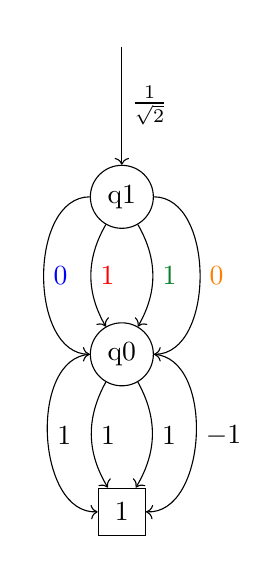
\begin{tikzpicture}[
        node distance=1.5cm,
        root/.style={circle,draw,minimum size=8mm},
        leaf/.style={rectangle,draw,minimum size=6mm},
        baseline={(current bounding box.center)}
      ]

        % terminal node
        \node[leaf] (t) at (0,0) {$1$};

        % nodes
        \node[root] (v) at (0,4) {q1};
        \node[root] (B) at (0,2) {q0};


        % incoming edge of weight 1
        \node[above=of v] (src) {};
        \draw[->] (src) -- node[right] {$\frac{1}{\sqrt{2}}$} (v);

        % four outgoing edges, one for each matrix entry (1,0,0,1)
        \draw[->] (v) edge[bend left=90]  node[right, text=orange]  {$0$} (B);
        \draw[->] (v) edge[bend left=30]  node[right, text=darkgreen]  {$1$} (B);
        \draw[->] (v) edge[bend right=30] node[right, text=red] {$1$} (B);
        \draw[->] (v) edge[bend right=90] node[right, text=blue] {$0$} (B);

        \draw[->] (B) edge[bend left=30]  node[right]  {$1$} (t);
        \draw[->] (B) edge[bend right=30] node[right] {$1$} (t);
        \draw[->] (B) edge[bend left=90]  node[right]  {$-1$} (t);
        \draw[->] (B) edge[bend right=90] node[right] {$1$} (t);


      \end{tikzpicture}
    \]
  \end{figure}
\end{frame}

\begin{frame}{QMDD para o vetor de estados}
  \begin{columns}[c]
    \begin{column}{.48\textwidth}
      \begin{itemize}
        \item Projeção da primeira coluna da matriz;
        \item Use a primeira e a terceira a resta para um qubit inicializado em \ket{0}.
      \end{itemize}
    \end{column}
    \begin{column}{.48\textwidth}
      \[
        X \otimes H \ket{00}
        =
        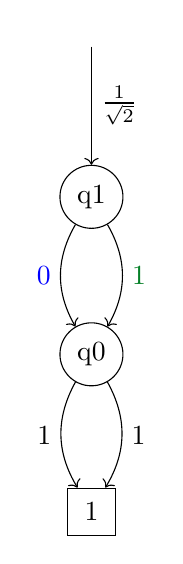
\begin{tikzpicture}[
          node distance=1.5cm,
          root/.style={circle,draw,minimum size=8mm},
          leaf/.style={rectangle,draw,minimum size=6mm},
          baseline={(current bounding box.center)}
        ]
      
          % terminal node
          \node[leaf] (t) at (0,0) {$1$};
      
          % nodes
          \node[root] (v) at (0,4) {q1};
          \node[root] (B) at (0,2) {q0};
      
      
          % incoming edge of weight 1
          \node[above=of v] (src) {};
          \draw[->] (src) -- node[right] {$\frac{1}{\sqrt{2}}$} (v);
      
          \draw[->] (v) edge[bend right=30] node[left, text=blue] {$0$} (B);
          \draw[->] (v) edge[bend left=30] node[right, text=darkgreen] {$1$} (B);
      
          \draw[->] (B) edge[bend right=30] node[left] {$1$} (t);
          \draw[->] (B) edge[bend left=30] node[right] {$1$} (t);
      
        \end{tikzpicture}
      \]
    \end{column}
  \end{columns}
\end{frame}

\begin{frame}{Porta controlada}
  \[
    \ket{0}_c\ket{\psi}_t
    \longrightarrow
    \ket{0}_c\ket{\psi}_t,
  \]
  \[
    \ket{1}_c\ket{\psi}_t
    \longrightarrow
    \ket{1}_cU\ket{\psi}_t.
  \]

  \begin{itemize}
    \item Controle em $\ket{0}$: aplica-se a identidade.
    \item Controle em $\ket{1}$: aplica-se a porta desejada.
  \end{itemize}

  \begin{exampleblock}{CNOT}
    Uma aresta leva à identidade; a outra leva à porta X.
  \end{exampleblock}
\end{frame}

\begin{frame}{Efeito das portas controladas no QMDD}
  \begin{center}
    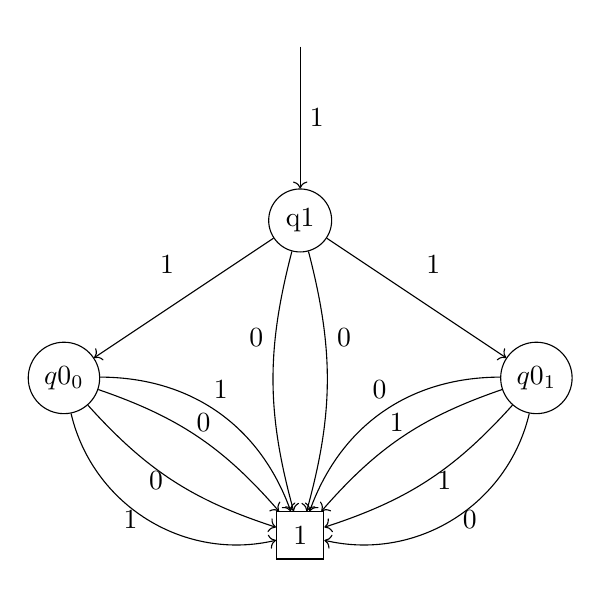
\begin{tikzpicture}[
      node distance=18mm,
      root/.style={circle,draw,minimum size=8mm},
      leaf/.style={rectangle,draw,minimum size=6mm},
      baseline={(current bounding box.center)}
    ]
  
      % terminal node
      \node[leaf] (t) at (3,0) {$1$};
  
      % nodes
      \node[root] (B) at (0,2) {$q0_0$};
      \node[root] (v) at (6,2) {$q0_1$};
      \node[root] (C) at (3,4) {q1};
  
  
      % incoming edge of weight 1
      \node[above=of C] (src) {};
      \draw[->] (src) -- node[right] {$1$} (C);
  
      \draw[->] (C) edge node[left, yshift=12pt] {$1$} (B);
      \draw[->] (C) edge[bend right=15] node[left, yshift=16pt] {$0$} (t);
      \draw[->] (C) edge[bend left=15] node[right, yshift=16pt] {$0$} (t);
      \draw[->] (C) edge node[right, yshift=12pt] {$1$} (v);
      
      % Control Qubit is 0. So Target must stay the same
      \draw[->] (B) edge[bend right=45] node[left] {$1$} (t);
      \draw[->] (B) edge[bend right=15]  node[left]  {$0$} (t);
      \draw[->] (B) edge[bend left=15]  node[right, xshift=-4pt, yshift=5pt]  {$0$} (t);
      \draw[->] (B) edge[bend left=35] node[right, yshift=8pt, xshift=-5pt] {$1$} (t);
  
      % Control Qubit is 1. So Target must be flipped
      \draw[->] (v) edge[bend right=35] node[left, yshift=8pt, xshift=5pt] {$0$} (t);
      \draw[->] (v) edge[bend right=15]  node[left, xshift=4pt, yshift=5pt]  {$1$} (t);
      \draw[->] (v) edge[bend left=15]  node[right]  {$1$} (t);
      \draw[->] (v) edge[bend left=45] node[right] {$0$} (t);
  
    \end{tikzpicture}
  \end{center}
  Cada qubit de controle duplica a quantia devértices no grafo.

\end{frame}

\begin{frame}{Implementação no Ket}
  Os algoritmos necessários foram implementados em Rust se baseando em propostas do QMDD na literatura

  \begin{columns}[t]
    \begin{column}{.48\textwidth}
      \begin{block}{Para o Ket}
        \begin{itemize}
          \item Construção de portas controladas.
          \item Multiplicação de QMDDs.
          \item Simulação forte
        \end{itemize}
      \end{block}
    \end{column}
    \begin{column}{.48\textwidth}
      \begin{block}{Necessário internamente}
        \begin{itemize}
          \item Identificação de vértices duplicados.
          \item Memoização de operações entre arestas.
          \item Adição de arestas.
          \item Normalização.
        \end{itemize}
      \end{block}
    \end{column}
  \end{columns}
\end{frame}

\begin{frame}{Aplicação de uma porta genérica}
  O estado atual é representado por um QMDD:
  \[
    \ket{\psi_{\text{novo}}}=U\ket{\psi_{\text{atual}}}.
  \]

  \begin{center}
    $\mathrm{QMDD}(U)\times\mathrm{QMDD}(\psi_{\text{atual}})$
  \end{center}

  \begin{itemize}
    \item A operação de multiplicação é recursiva.
    \item O método visita vértices e arestas até chegar ao terminal.
    \item Pares de arestas já calculados são reutilizados pela memoização.
  \end{itemize}
\end{frame}

\begin{frame}{Simulação forte e cálculo de probabilidade}
  \textbf{Recuperação do vetor de amplitudes}
  \begin{itemize}
    \item Percorrer todos os caminhos da aresta inicial ao terminal.
    \item Multiplicar os pesos de cada caminho.
    \item Associar o produto ao estado correspondente da base computacional.
  \end{itemize}

  \textbf{Cálculo de probabilidade}
  \begin{itemize}
    \item Somar a probabilidade acumulada de cada vértice do qubit
    \item Acumular a probabilidade da subárvore de cada vértice do qubit
  \end{itemize}
\end{frame}

\begin{frame}{Medição}
\textbf{Medição destrutiva}
  \[
    M_0=
    \begin{bmatrix}
      1&0\\
      0&0
    \end{bmatrix},
    \qquad
    M_1=
    \begin{bmatrix}
      0&0\\
      0&1
    \end{bmatrix}.
  \]
  
  \begin{itemize}
    \item Aplicar $M_0$ ou $M_1$ para \ket{0} ou \ket{1} respectivamente
    \item Renormalizar o estado de acordo com a probabilidade calculada previamente
  \end{itemize}
\end{frame}

\begin{frame}{Testes da implementação}
  \begin{itemize}
    \item Avaliação manual de circuitos pequenos.
    \item Criação de estados de Bell e colapso do estado entrelaçado.
    \item Circuito de três qubits com controles em posições diferentes do alvo.
    \item Medição sucessiva de um mesmo qubit.
  \end{itemize}

  \begin{exampleblock}{Validação}
    Os resultados foram comparados ao simulador denso do Ket e apresentaram compatibilidade em diferentes algoritmos.
  \end{exampleblock}
\end{frame}

\begin{frame}{Experimentos realizados}
  Comparação entre:
  \begin{columns}[c]
    \begin{column}{.48\textwidth}
      Simuladores
      \begin{itemize}
        \item QMDD;
        \item Denso;
        \item Esparso.
      \end{itemize}
    \end{column}
    \begin{column}{.48\textwidth}
      Algoritmos:
      \begin{itemize}
        \item Grover;
        \item FALQON;
        \item Estimação de Fase Quântica.
      \end{itemize}
    \end{column}
  \end{columns}

  Dois tipos de variação:
  \begin{enumerate}
    \item Número de qubits.
    \item Número de camadas do FALQON.
  \end{enumerate}
\end{frame}

\begin{frame}{Algoritmos utilizados}
  \begin{block}{Grover}
    Busca em conjuntos desordenados. Utiliza repetidamente portas X, H e portas Z controladas.
  \end{block}

  \begin{block}{FALQON}
    Otimização por feedback aplicada ao problema Max-Cut. Possui menos controles que Grover e utiliza sucessivamente portas controladas sobre os mesmos qubits.
  \end{block}

  \begin{block}{Estimação de Fase Quântica}
    Estima a fase de um operador e combina portas controladas com a Transformada Quântica de Fourier.
  \end{block}
\end{frame}

\begin{frame}{Resultado --- Grover}
  \begin{center}
    \includegraphics[width=.86\textwidth,height=.68\textheight,keepaspectratio]{grover_by_qubits.png}
  \end{center}

  O QMDD foi competitivo até aproximadamente 14 qubits. A partir desse ponto, o crescimento dos controles aumentou rapidamente o tempo de execução.
\end{frame}

\begin{frame}{Resultado --- FALQON por qubits}
  \begin{center}
    \includegraphics[width=.86\textwidth,height=.68\textheight,keepaspectratio]{falqon_by_qubits.png}
  \end{center}

  Aos 18 qubits, QMDD e esparso tiveram tempos próximos. O QMDD manteve-se competitivo em um intervalo maior que no Grover.
\end{frame}

\begin{frame}{Resultado --- Estimação de Fase Quântica}
  \begin{center}
    \includegraphics[width=.86\textwidth,height=.68\textheight,keepaspectratio]{qpe_by_qubits.png}
  \end{center}

  O simulador denso chegou a 30 qubits. O esparso chegou a 27 qubits, enquanto o QMDD deixou de concluir a partir de 21 qubits.
\end{frame}

\begin{frame}{Variação do número de camadas no FALQON}
  \begin{itemize}
    \item Número de qubits fixado em 18.
    \item Primeira execução a partir de 250 camadas.
    \item Experimentos posteriores aumentaram o número de camadas.
  \end{itemize}

  Como a largura do circuito permanece constante, o objetivo é observar o custo provocado pelo aumento da profundidade.
\end{frame}

\begin{frame}{Resultado --- camadas do FALQON}
  \begin{center}
    \includegraphics[width=.86\textwidth,height=.68\textheight,keepaspectratio]{falqon_by_layers.png}
  \end{center}

  O tempo do QMDD cresceu aproximadamente de forma linear. A partir de cerca de 1500 camadas, ele passou a superar o simulador denso.
\end{frame}

\begin{frame}{Conclusões}
  \begin{itemize}
    \item O QMDD é competitivo em circuitos com padrões repetidos e poucos controles.
    \item O crescimento do número de vértices reduz essa vantagem em circuitos altamente controlados.
    \item O simulador denso se beneficia da paralelização em arquiteturas com vários núcleos.
    \item O QMDD tende a ser relativamente mais vantajoso em dispositivos com menos núcleos.
  \end{itemize}

  \begin{exampleblock}{Objetivo geral atingido}
    Um simulador QMDD foi implementado e integrado ao Ket, podendo ser escolhido como opção de execução.
  \end{exampleblock}
\end{frame}

\begin{frame}{Limitações e trabalhos futuros}
  \begin{block}{Baixa paralelização}
    Operações recursivas sobre vértices e arestas dificultam a distribuição segura entre núcleos.
  \end{block}

  \begin{block}{Memória}
    Vértices não alcançados não são removidos imediatamente, podendo aumentar o consumo de memória.
  \end{block}

  \begin{block}{LIMDD}
    Estender o trabalho para o \emph{Local Invertible Map Decision Diagram}, que usa matrizes invertíveis locais nas arestas.
  \end{block}
\end{frame}

\begin{frame}{Referências}
  \begin{thebibliography}{9}

    \bibitem{nisq}
      Michael A. Nielsen e Isaac L. Chuang.
      \emph{Quantum Computation and Quantum Information}.
      Cambridge University Press, 2010.

    \bibitem{qmdd}
      D. Michael Miller e Mitchell A. Thornton.
      \emph{QMDD: A Decision Diagram Structure for Representing and
      Manipulating Quantum Circuits}.
      International Workshop on Spectral Logic and Applications, 2006.

    \bibitem{ket}
      \emph{Ket Quantum Programming Platform}.
      Documentação oficial da biblioteca de programação quântica.

  \end{thebibliography}
\end{frame}

\contato{Contato: \\ \url{gabriel.sartori@grad.ufsc.br}}
\capadetras{Obrigado!}

\end{document}
